\documentclass[UTF8,a4paper,11pt]{ctexart}
\usepackage[margin=22mm,headheight=14pt,footskip=12mm]{geometry}
\usepackage{amsmath,amssymb,array,longtable,booktabs,tikz,graphicx,needspace,enumitem,fancyhdr,hyperref}
\usetikzlibrary{arrows.meta,positioning,calc,shapes.geometric,fit}
\newsavebox{\StudyDiagramBox}
\usepackage{microtype}
\hypersetup{colorlinks=false,pdfborder={0 0 0},pdfauthor={Good Learning},bookmarks=false}
\newfontfamily\circledfont{Segoe UI Symbol}
\newcolumntype{P}[1]{>{\raggedright\arraybackslash}p{#1}}
\setlength{\LTleft}{0pt}\setlength{\LTright}{0pt}
\setlength{\parindent}{0pt}\setlength{\parskip}{.65em}
\linespread{1.18}
\raggedbottom
\setcounter{secnumdepth}{0}
\setlist{leftmargin=2.2em,itemsep=.4em,topsep=.5em}
\ctexset{section={format=\Large\bfseries\sffamily,beforeskip=1.35em,afterskip=.65em},
subsection={format=\large\bfseries\sffamily,beforeskip=1em,afterskip=.45em}}
\newcommand{\chaptertitle}[1]{\Needspace{8\baselineskip}\noindent{\LARGE\bfseries\sffamily #1}\par\vspace{4mm}\hrule\vspace{6mm}}
\newcommand{\CompactQuestion}[2]{\par\Needspace{5\baselineskip}\noindent\textbf{#1.}\ #2\par\vspace{.8em}}
\newcommand{\PracticeQuestion}[3]{\par\Needspace{4\baselineskip}\noindent\begin{minipage}{\linewidth}\textbf{#1.}\ #2\par\noindent\rule{0pt}{#3mm}\par\end{minipage}\par}
\newcommand{\CompactQuestionColon}[2]{\par\Needspace{5\baselineskip}\noindent\textbf{#1：}\ #2\par\vspace{.8em}}
\newcommand{\QuestionSpace}[1]{\par\noindent\rule{0pt}{#1mm}\par}
\newcommand{\PracticeQuestionColon}[3]{\par\Needspace{4\baselineskip}\noindent\begin{minipage}{\linewidth}\textbf{#1：}\ #2\par\noindent\rule{0pt}{#3mm}\par\end{minipage}\par}
\pagestyle{fancy}\fancyhf{}\fancyfoot[C]{\thepage}\renewcommand{\headrulewidth}{0pt}
\begin{document}

\chaptertitle{教学配图示例}
以下是新编的绘图验证材料，不计入学习进度。使用现成 TikZ/PGF 引擎；各图可按当前课程修改。

\section{1. 负反馈系统方框图}
假设各环节为线性时不变系统，使用零初始条件下的传递函数。$R(s)$ 是给定输入，$Y(s)$ 是输出；$G_c(s)$ 是控制器，$G_p(s)$ 是被控对象，$H(s)$ 是反馈环节。

\begin{lrbox}{\StudyDiagramBox}
\begin{tikzpicture}[>=Stealth,thick,font=\small,
 block/.style={draw,minimum width=18mm,minimum height=11mm},
 sum/.style={draw,circle,minimum size=8mm,inner sep=0pt}]
\node[sum] (sum) at (1.5,0) {};
\node[block] (gc) at (4,0) {$G_c(s)$};
\node[block] (gp) at (7,0) {$G_p(s)$};
\coordinate (take) at (9.1,0);
\node[block] (h) at (6,-2) {$H(s)$};
\draw[->] (-.2,0) node[left] {$R(s)$} -- (sum.west);
\node at (1.00,.35) {$+$};
\node at (1.83,-.52) {$-$};
\draw[->] (sum.east) -- node[above] {$E(s)$} (gc.west);
\draw[->] (gc.east) -- node[above] {$U(s)$} (gp.west);
\draw[->] (gp.east) -- (10.6,0) node[right] {$Y(s)$};
\fill (take) circle (1.6pt);
\draw[->] (take) |- (h.east);
\draw[->] (h.west) -| node[pos=.25,above] {$B(s)$} (sum.south);
\node[below=2mm of gc] {控制器};
\node[below=2mm of gp] {被控对象};
\node[below=2mm of h] {反馈环节};
\end{tikzpicture}
\end{lrbox}
\par\begin{center}
\ifdim\wd\StudyDiagramBox>\linewidth
\resizebox{\linewidth}{!}{\usebox{\StudyDiagramBox}}
\else\usebox{\StudyDiagramBox}\fi
\end{center}\par
图 1：圆圈是求和点，实心点是取样点。沿上方箭头读前向传递，再从输出取样点沿下方回路返回；返回信号从负号输入求和点。

按图逐项写出关系：$B=HY$，$E=R-B$，$U=G_cE$，$Y=G_pU$。图中每一条关系均使用同一组信号符号，因此有

\[Y=G_cG_p(R-HY),\qquad \frac{Y(s)}{R(s)}=\frac{G_c(s)G_p(s)}{1+G_c(s)G_p(s)H(s)}.\]
负反馈的符号来自求和点。闭环传递函数表达式本身不能保证系统稳定；稳定性还需根据具体环节检查。

\section{2. 同一系统的信号流图}
信号流图用节点表示变量，用有向支路表示乘以某个增益。进入同一节点的各支路贡献相加。因此，方框图求和点的负号在这里写进反馈支路增益。

\begin{lrbox}{\StudyDiagramBox}
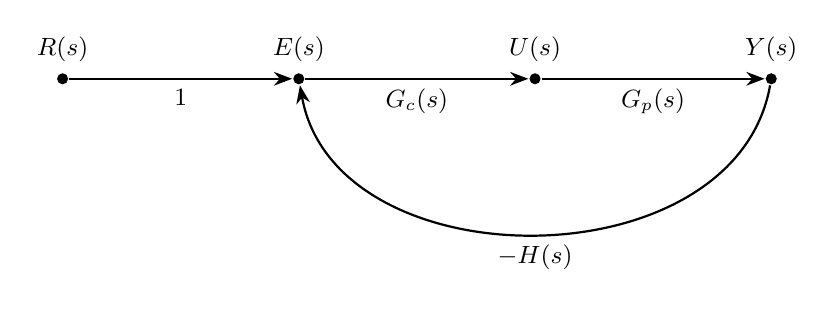
\begin{tikzpicture}[>=Stealth,thick,font=\small,
 signal/.style={circle,fill=black,inner sep=0pt,minimum size=4pt}]
\node[signal,label=above:$R(s)$] (r) at (0,0) {};
\node[signal,label=above:$E(s)$] (e) at (3,0) {};
\node[signal,label=above:$U(s)$] (u) at (6,0) {};
\node[signal,label=above:$Y(s)$] (y) at (9,0) {};
\draw[->] (r) -- node[below] {$1$} (e);
\draw[->] (e) -- node[below] {$G_c(s)$} (u);
\draw[->] (u) -- node[below] {$G_p(s)$} (y);
\draw[->] (y) to[out=-100,in=-80,looseness=1.1]
 node[pos=.5,below] {$-H(s)$} (e);
\end{tikzpicture}
\end{lrbox}
\par\begin{center}
\ifdim\wd\StudyDiagramBox>\linewidth
\resizebox{\linewidth}{!}{\usebox{\StudyDiagramBox}}
\else\usebox{\StudyDiagramBox}\fi
\end{center}\par
图 2：从 $Y$ 返回 $E$ 的支路增益为 $-H$。两个进入 $E$ 的贡献是 $R$ 和 $-HY$，所以仍有 $E=R-HY$，与图 1 一致。

这张图只有一条前向通路，增益为 $P=G_cG_p$；只有一个回路，回路增益为 $L=-G_cG_pH$。因此闭环结果是 $P/(1-L)=G_cG_p/(1+G_cG_pH)$。这也提供了两种画法是否表达同一个系统的核对方法。

\section{3. 栈的入栈与出栈状态}
本例采用容量为 4 的顺序栈，索引从下往上增加；$top$ 指向当前栈顶元素，空栈时 $top=-1$。方格中的“空”表示不属于栈的有效区域，不要求底层存储单元已经清零。

\begin{lrbox}{\StudyDiagramBox}
\begin{tikzpicture}[>=Stealth,thick,font=\small]
\foreach \shift/\title in {0/初始状态,4.2/入栈后,8.4/出栈后} {
  \begin{scope}[xshift=\shift cm]
  \node[font=\bfseries] at (.65,3.35) {\title};
  \foreach \i in {0,1,2,3} {
    \draw (0,.65*\i) rectangle (1.3,.65*\i+.65);
    \node[left] at (-.1,.65*\i+.325) {\i};
  }
  \node at (.65,.325) {10};
  \node at (.65,.975) {20};
  \node at (.65,2.275) {空};
  \node[below] at (.65,-.1) {栈底};
  \end{scope}
}
\node at (.65,1.625) {空};
\node at (4.85,1.625) {30};
\node at (9.05,1.625) {空};
\draw[->] (2.1,.975) node[right] {$top=1$} -- (1.3,.975);
\draw[->] (6.3,1.625) node[right] {$top=2$} -- (5.5,1.625);
\draw[->] (10.5,.975) node[right] {$top=1$} -- (9.7,.975);
\draw[->] (1.6,2.9) -- node[above] {push(30)} (4,2.9);
\draw[->] (5.8,2.9) -- node[above] {pop()} (8.2,2.9);
\node at (9.05,-.85) {返回值：30};
\end{tikzpicture}
\end{lrbox}
\par\begin{center}
\ifdim\wd\StudyDiagramBox>\linewidth
\resizebox{\linewidth}{!}{\usebox{\StudyDiagramBox}}
\else\usebox{\StudyDiagramBox}\fi
\end{center}\par
图 3：初始有效内容自栈底到栈顶为 $[10,20]$。push(30) 使 $top$ 从 1 变为 2，并在索引 2 写入 30；pop() 先取出索引 2 的 30 作为返回值，再使 $top$ 回到 1。最终有效内容恢复为 $[10,20]$。

此处三幅图使用同一方向、容量和索引，读者可以直接比较变化。若另一份教材用 $top$ 指向下一空位，就必须同时更改指针标注和操作解释，不能混用两种定义。

\end{document}
